\documentclass[]{article}

% Get better typography
\usepackage[protrusion=true,expansion=true]{microtype}		

% For algorithms
\usepackage[boxruled,linesnumbered,vlined,inoutnumbered]{algorithm2e}
\SetKwInOut{Parameter}{Parameters}

% For basic math, align, fonts, etc.
\usepackage{amsmath}
\usepackage{amsthm}
\usepackage{amssymb}
\usepackage{mathtools}
\usepackage{mathrsfs}
\usepackage{rotating}
\usepackage{gensymb} % For \degree
\usepackage{enumitem} %for enumerating with letters


\newtheorem{defn}{Definition}[]
\newtheorem{thm}{Theorem}[]
\newtheorem{claim}{Claim}[]
\newtheorem{lemma}{Lemma}[]
\newtheorem{prop}{Property}[]
\newtheorem{ass}{Assumption}[]
\newtheorem{cor}{Corollary}[]

\DeclareMathOperator*{\argmin}{arg\,min}
\DeclareMathOperator*{\argmax}{arg\,max}

\usepackage{courier} % For \texttt{foo} to put foo in Courier (for code / variables)
\usepackage{lipsum} % For dummy text

% For images
\usepackage{graphicx}
\usepackage{subcaption}
\usepackage[space]{grffile} % For spaces in image names

% For bibliography
\usepackage[round]{natbib}

% For color
\usepackage{xcolor}
\definecolor{light-grey}{rgb}{0.95,0.95,0.95}
\definecolor{dark-red}{rgb}{0.4,0.15,0.15}
\definecolor{dark-blue}{rgb}{0,0,0.7}

% For questions and answers
\usepackage[framemethod=tikz]{mdframed}
\newtheorem{question}{Question}
\mdfdefinestyle{que}{
  linecolor=dark-blue,
  backgroundcolor=white!20,
}
\surroundwithmdframed[style=que]{question}
\newtheorem{answer}{Answer}
\mdfdefinestyle{ans}{
  linecolor=dark-red,
  backgroundcolor=white!20
  % , rotatebox
}
\surroundwithmdframed[style=ans]{answer}
\usepackage{environ}
\NewEnviron{Answer}
{%
\noindent
\rotatebox[origin=c]{180}{%
\noindent
\begin{minipage}[t]{\linewidth}
\begin{answer}
\BODY
\end{answer}%
\end{minipage}%
}%
}%

% Only show sections in table of contents and rename
\setcounter{tocdepth}{2}
\renewcommand{\contentsname}{Table of Contents}

% For links (e.g., clicking a reference takes you to the phy)
\usepackage{hyperref}
\hypersetup{
    colorlinks, linkcolor={dark-blue},
    citecolor={dark-blue}, urlcolor={dark-blue}
}

%-------------------------
%	TOGGLE ANSWER VISIBILITY
%-------------------------
\newif\ifHomeworkOneAnswers
\HomeworkOneAnswersfalse
%\HomeworkOneAnswerstrue

%-------------------------
%	BEGIN DOCUMENT / TITLE
%-------------------------

\begin{document}
%-----------------
%	Homework 2
%-----------------
\newpage
\begin{center}
    \begin{Large}
    CMPSCI 687 Homework 2
    \end{Large}
    \\
    Due October 3, 2018, 11:55pm Eastern Time
\end{center}
\addcontentsline{toc}{subsection}{\textbf{Homework 2}}

\noindent {\bf Instructions: } This homework  consists of a programming portion only. Collaboration is not allowed on any part of this assignment. Submissions must be typed (hand written and scanned submissions will not be accepted). You must use \LaTeX. The coding portion of the assignment should be submitted on Gradescope as a .zip file containing your code (see details below). The written response answers should be submitted to Gradescope via a .pdf file and a tagged with the relevant pages. You \textbf{must} use the template we have provided, which is located at the github repository \href{https://github.com/bmetevier/rl-framework-687-public}{here}. You may not use any reinforcement learning or machine learning specific libraries in your code, e.g., TensorFlow or PyTorch (you may use libraries like numpy and matplotlib though). If you are unsure whether you can use a library, ask on Piazza. The automated system will not accept assignments after 11:55pm on October 3. The tex file for this homework can be found \href{https://people.cs.umass.edu/~pthomas/courses/CMPSCI_687_Fall2019/hw2Source.tex}{here}. The number of points for this assignment is 100. 

\section*{Implement Cart-Pole}

In this assignment you will implement the cart-pole domain using the (frictionless) dynamics described by \citet[Equations 23 and 24]{Florian2007}, we provide the expressions below. 
%When implementing cart-pole, the state should include the position of the cart, velocity of the cart, angle of the pole, and angular velocity of the pole. 
You \textbf{must} use a forward Euler approximation of the dynamics. If the cart hits the boundary of the track, the pole falls below a fail angle, or the time limit is exceeded, then terminate the episode.
%
\textbf{You may not use existing RL code for this problem---you must implement the agent and environment entirely on your own and using the class template.} 

The Cart-pole environments consists of two interacting bodies: a cart with position $x$ and velocity $\dot x$, and a pole with angle $\theta$ and angular velocity $\dot \theta$. 
%
An expression for the pole's angular acceleration is 
%
\begin{equation}
    \ddot \theta = \frac{g \sin{\theta} + \cos{\theta}\left( \frac{-F-m_p l \dot \theta^2 \sin \theta}{m_c + m_p}\right )}{l \left ( \frac{4}{3} - \frac{m_p \cos^2{\theta}}{m_c + m_p}\right )},
\end{equation}
%
where $g$ is the acceleration due to gravity, $F$ is the force applied to the cart, $m_p$ is the mass of the pole, $m_c$ is the mass of the cart, and $l$ is half the length of the pole. 
%
An expression for acceleration of the cart is 
%
\begin{equation}
    \ddot x = \frac{F + m_p l (\dot \theta^2 \sin{\theta} - \ddot \theta \cos{\theta})}{m_c + m_p}.    
\end{equation}
%
The system state is described by the state vector $\mathbf{x} \coloneqq [x, v, \theta, \omega ]$, where $v = \dot x$ and $\omega = \dot \theta$. 

The state space equations of motion are:
%
\begin{align}
    \dot x_{t} = &\ v_t \\
    \dot v_{t} = &\ \frac{F + m_p l (\dot \theta_t^2 \sin{\theta_t} - \dot \omega_t \cos{\theta_t})}{m_c + m_p} \\
    \dot \theta_t = &\ \omega_t \\
    \dot \omega_t = &\ \frac{g \sin{\theta_t} + \cos{\theta_t}\left( \frac{-F-m_p l \omega_t^2 \sin \theta_t}{m_c + m_p}\right )}{l \left ( \frac{4}{3} - \frac{m_p \cos^2{\theta_t}}{m_c + m_p}\right )}.
\end{align}
%
Using the Euler approximation the system evolves as:
\begin{equation}
    \mathbf{x}_{t+1} = \mathbf{x}_t + \Delta t \dot {\mathbf{x}}_t,
\end{equation}
where $\dot {\mathbf{x}}_t = [\dot x_t, \dot v_t, \dot \theta_t, \dot \omega_t]$ and $\Delta t$ is the time in seconds between updates. 
%
In this environment, an agent's action specifies a force $F \in [-F_\text{mag}, F_\text{mag}]$ on the cart. Traditionally, in RL, the cart pole environment is specified with two discrete actions, where $a_0 = -F_\text{mag}$ and $a_1 = F_\text{mag}$. You must use this action space in creating the environment.

Use the following values for the cart-pole constants:
\begin{itemize}
    \item Fail angle $= \pi/12$. (If it exceeds this value or its negative, the episode ends in failure.)
    \item Cart boundaries are at $x=-3m$ and $x=3m$.
    \item Max motor force magnitude $F_\text{mag} = 10.0$ (force on cart in Newtons).
    \item Gravitational constant $g$ is $9.8$.
    \item Cart mass $m_c = 1.0 \text{ kg}$.
    \item Pole mass $m_p = 0.1 \text{ kg}$.
    \item Pole half-length $l = 0.5m$.
    \item $\Delta t = 0.02\text{ seconds}$ (time step).
    \item Max time before end of episode $= 20\text{ seconds}$.
\end{itemize}

\section*{Genetic Algorithms}
Genetic algorithms (GAs) are a family of biologically inspired BBO algorithms that are empirically competitive with deep reinforcement learning methods \citep{such2017deep}. Intuitively, the GA starts with a population of \emph{candidate solutions} (in our case, parameterized policies $\theta$) and iteratively modifies, or evolves, the population. We call the number of iterations over which a population is evolved the number of \emph{generations}. 

At every generation, the GA uses three main methods, called \emph{genetic operators}, to create the next generation. These genetic operators are known as parent selection, mutation operators, and crossover operators. \emph{Parent selection} chooses which candidate solutions in the current generation will be used as parents for creating children in the next generation.  \emph{Mutation operators} apply random changes to parents to create children for the next generation. \emph{Crossover operators} combine two or more parents to create children for the next generation.

Example pseudocode for a simple GA is below. Pseudocode for the functions \texttt{get\_parents} and \texttt{get\_children} are purposefully not provided. At each generation, every candidate solution, $\theta_i$, in the population, $P=\{\theta_i\}_{i=0}^K$, is evaluated and a \emph{fitness score} for $\theta_i$ is produced. The top $K_p$ candidate solutions are then chosen to become parents of the next generation (this parent selection method is known as truncation selection). Children are created by selecting a parent uniformly at random to mutate by applying additive Gaussian noise to the parent: $\theta_{\text{child}} = \theta_{\text{parent}} + \alpha\epsilon$, where $\epsilon \sim \mathcal N(0,1)$ and $\alpha$ is a hyperparameter. $K_e$ candidate solutions in the new generation are unmodified copies of the top $K_e$ candidate solutions from the previous generation. This is known as \emph{elitism}. 
\\
\begin{algorithm}[H]
    \For{$g=1$ \KwTo $G$}{
        \For{$k=1$ \KwTo $K$}{
            $\hat J_k = \texttt{evaluate}(\theta_k, N)$\;
        }
        $\texttt{sorted} = \texttt{sort}((\theta_1,\hat J_1), (\theta_2,\hat J_2),\dotsc, (\theta_K, \hat J_K), \text{descending})$\;
        %
        $\texttt{parents} =  \texttt{get\_parents}(K_p, \texttt{sorted})$\;
        %
        $\texttt{next\_gen} = \texttt{sorted}[1:K_e].\texttt{append}(\texttt{get\_children}(\alpha, \texttt{parents}))$\;
    }
\caption{\texttt{Genetic Algorithm} (GA) for Policy Search.\newline
\textbf{Input:}
\newline \textbf{1)} Number of generations, $G \in \mathbb N_{>1}$ [for example, $G=300$]
\newline \textbf{2)} Initial population, $P = \{\theta_i\}_{i=0}^K$
\newline \textbf{3)} Population size, $K \in \mathbb N_{>1}$ [for example, $K=20$]
\newline \textbf{4)} Truncation index, $K_p \in \mathbb N_{>0}$, where $K_p < K$ [for example, $K_p=10$]
\newline \textbf{5)} Elite population, $K_e \in \mathbb N_{>0}$, where $K_e < K$ [for example, $K_e=10$]
\newline \textbf{6)} Number of episodes to sample per policy, $N \in \mathbb N_{>0}$ [for example, $N=10$]
\newline \textbf{7)} Learning parameter $\alpha \in \mathbb R$ [for example, $\alpha=2.5$]}
\label{alg:crossEntropy}
\end{algorithm}

\begin{algorithm}[H]
    Run the parameterized policy using policy parameters $\theta$ for $N$ episodes\;
    Compute the resulting $N$ returns, $G^1,G^2,\dotsc,G^N$, where
    $
    G^i = \sum_{t=0}^\infty R_t^i.
    $\;
    Return $\frac{1}{N}\sum_{i=1}^N G^i$\;
\caption{\texttt{evaluate}\newline
\textbf{Input:}
\newline \textbf{1)} Policy parameter vector, $\theta \in \mathbb R^n$
\newline \textbf{2)} Number of episodes to sample, $N \in \mathbb N_{>0}$ [for example, $N=10$]}
\label{alg:evaluate}
\end{algorithm}
\textbf{Note} that we do not provide pseudocode for the \texttt{get\_parents} and \texttt{get\_children} methods. It will be up to you to define these methods.  

\section*{Problems}
Six questions ask for a plot. You must report two plots: one for cart-pole and one for 687-Gridworld, where each of these two plots has a curve corresponding to the cross-entropy method, a curve corresponding to the GA method, and a curve corresponding to first-choice hill-climbing. In the coding problems your solutions will be graded via an autograder on Gradescope. To submit assignments you must zip the rl687 folder and its structure must be the same as the template. You must use the same files provided in the template and fill in the missing function bodies. Correct solutions can be fit within the provided files, but you can create additional files as necessary for the assignment. However, if any errors occur in using them the questions will be marked as zero. The functions will need to match our outputs exactly so pay attention to types (we use np.float64 and np.int for arrays, int, float, and bool else where). The autograder will give results before the assignment is due so you can check your implementations for correctness. 
\\\\
\noindent \textbf{Coding Problems:}

\begin{enumerate}
    
    \item{(15 Points) Implement the cart-pole environment as specified above.}
    
    \item{(5 Points) Implement the tabular softmax policy.}
    
    \item{(10 Points) Implement the cross-entropy method as described in the class notes.}
    
    \item{(10 Points) Implement the First-choice hill-climbing algorithm as described in the class notes.}
    
    \item{(10 Points) Implement the GA algorithm described earlier in this assignment.}
\end{enumerate}

\noindent\textbf{Written Response:}

\begin{enumerate}
    \item (7.5 Points) Apply the CEM algorithm to the More-Watery 687-Gridworld. Use a tabular softmax policy. Search the space of hyperparameters for hyperparameters that work well. Report how you searched the hyperparameters, what hyperparameters you found worked best, and present a learning curve plot using these hyperparameters, as described in class. This plot may be over any number of episodes, but should show convergence to a nearly optimal policy. The plot should average over at least $500$ trials and should include standard deviation error bars.  \\
    \textbf{Answer:}\\
    To search the hyperparameters, I first set the range for all parameters, and initialized these hyperparameters using \textit{np.linspace} which will generate a sequence of all possible choices in that specific range. Then I will randomly select one from each parameters for every trail. All returns obtained from episodes will be collected and returned to plot the learning rate. The algorithm returns a best set of hyperparameter after 10 random searches. The hyperparameters are: 'sigma': 1.625, 'popSize': 40, 'numElite': 4, 'numEpisodes': 30, 'epsilon': 1.625. The learning curve for problem 1 is attached below:
    \begin{figure}[htbp]
        \centering
        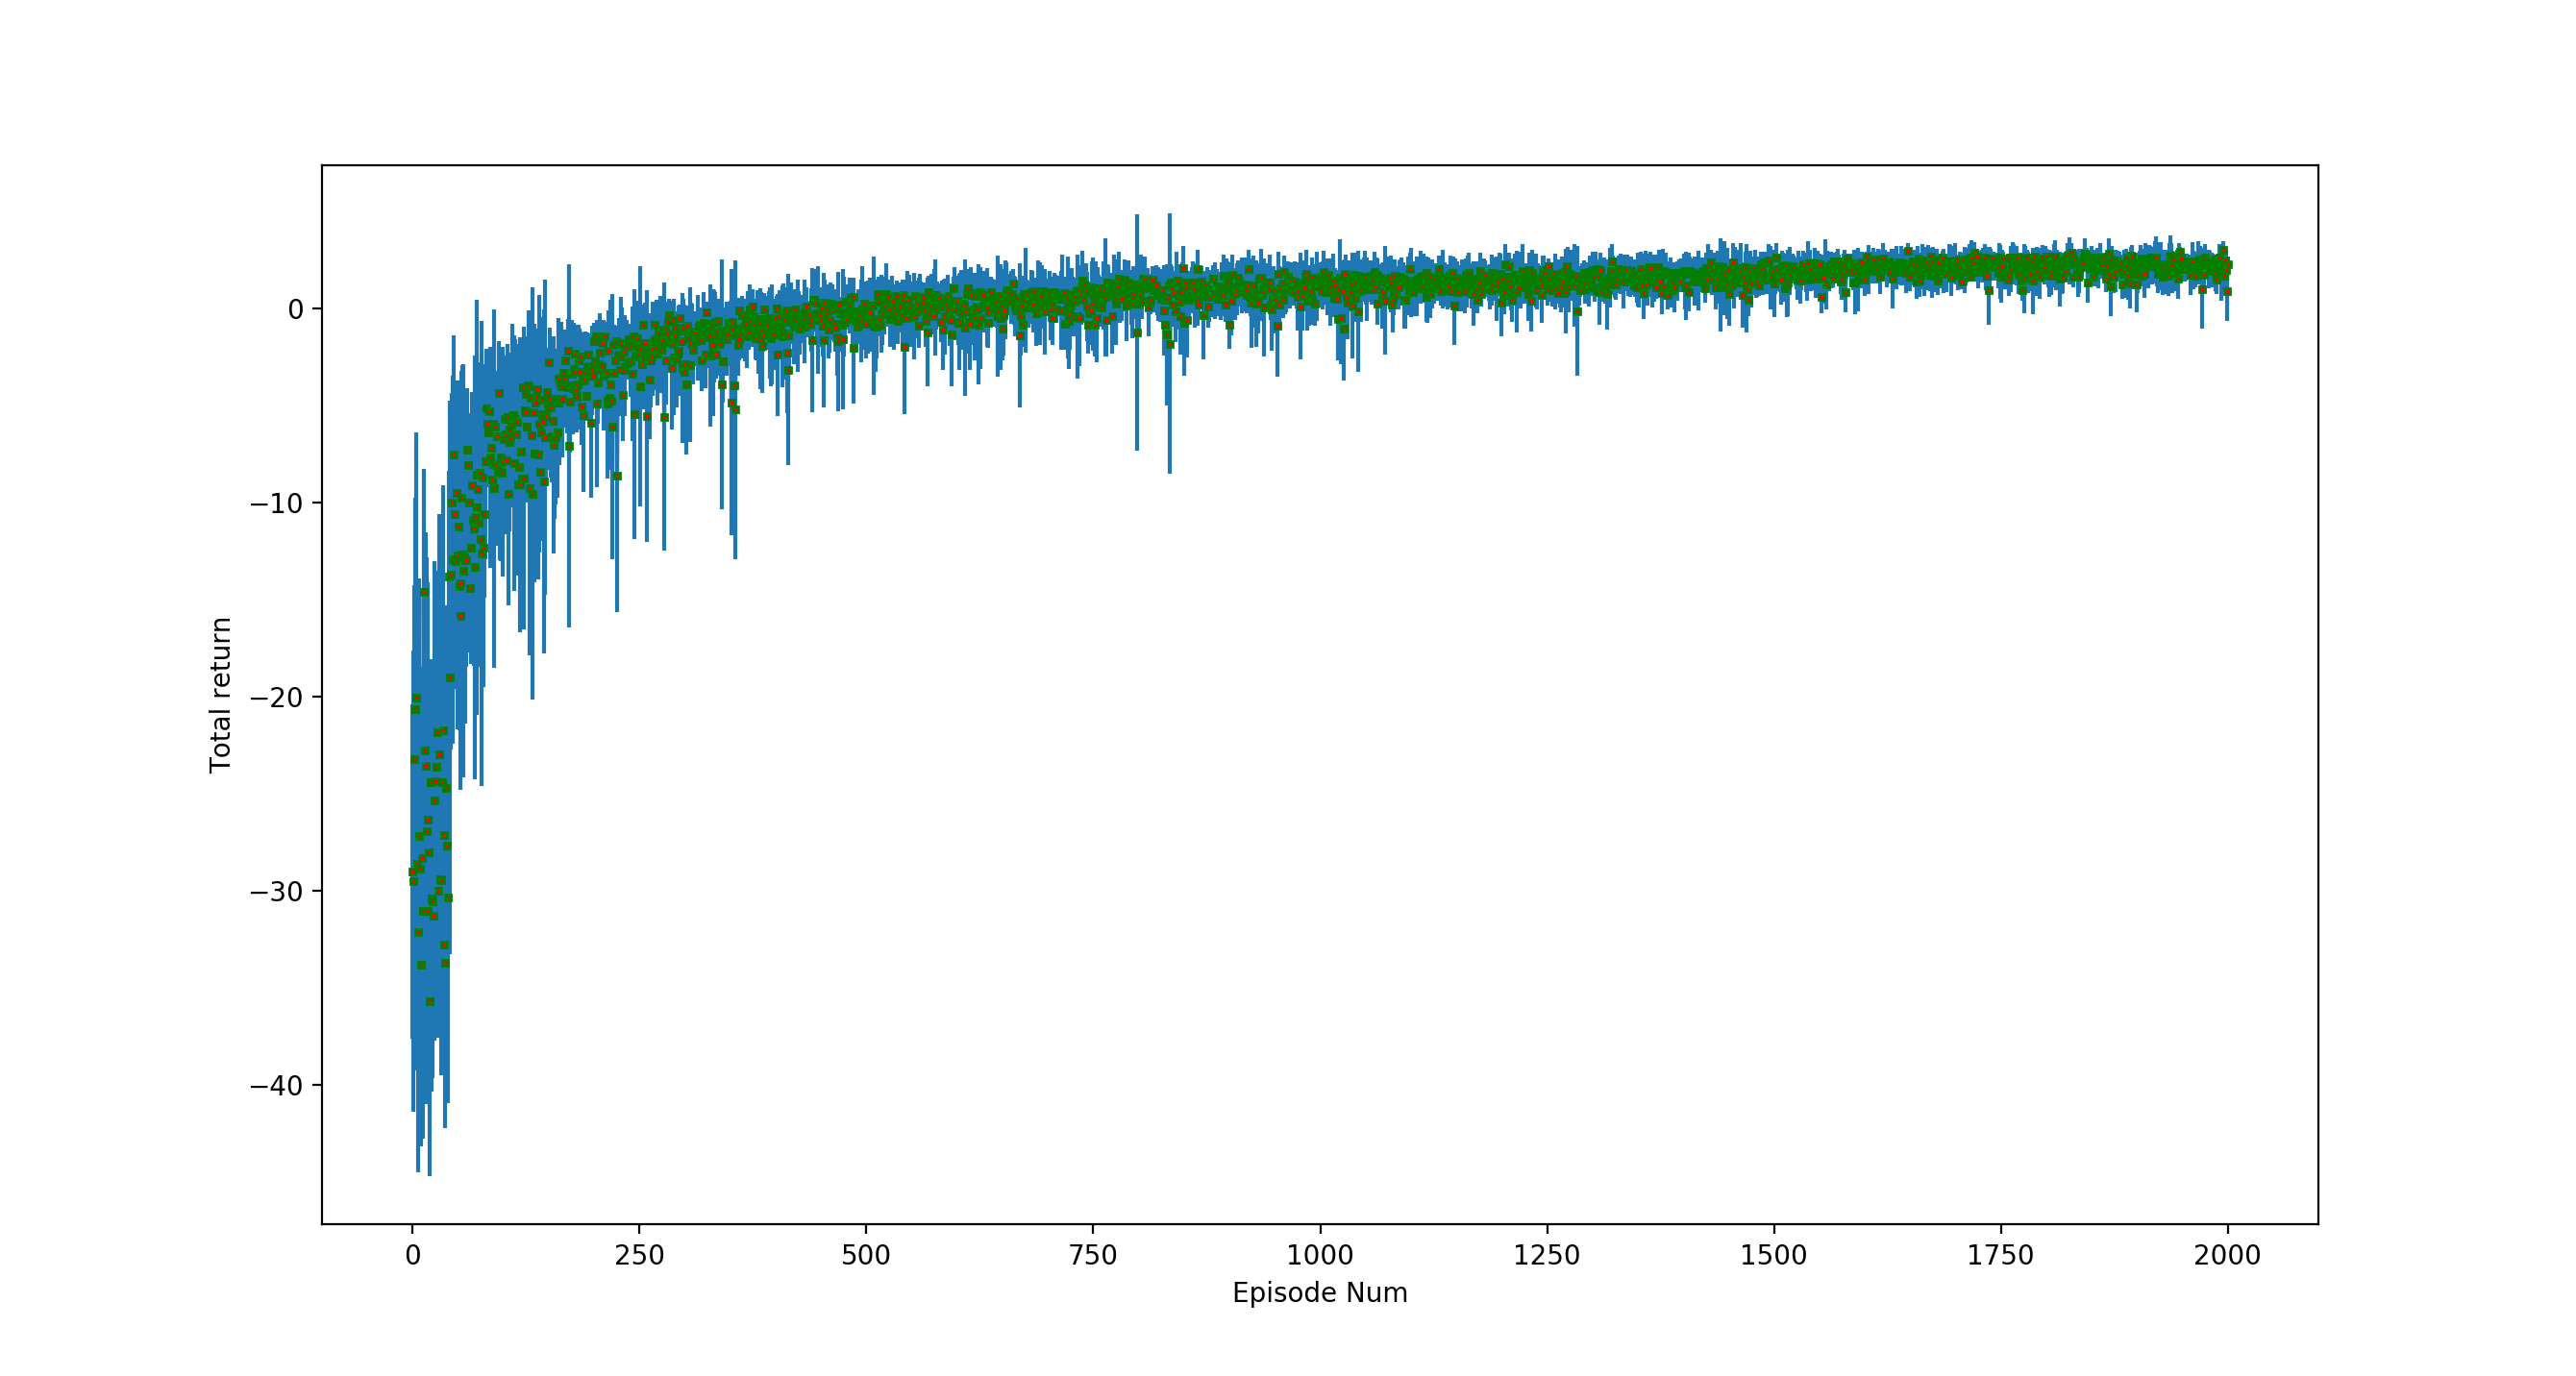
\includegraphics[height=6.0cm,width=9.5cm]{p1.png}
        \caption{Learning Curve for Problem 1}
    \end{figure}

    \item (7.5 Points) Repeat the previous question, but using first-choice hill-climbing on the More-Watery 687-Gridworld domain. Report the same quantities.  \\
    \textbf{Answer:}\\
    Searching strategy is the same. The best hyperparameters are :"sigma": 1.625, "numEpisodes": 30. The learning curve for problem 2 is attached below:
    \begin{figure}[htbp]
        \centering
        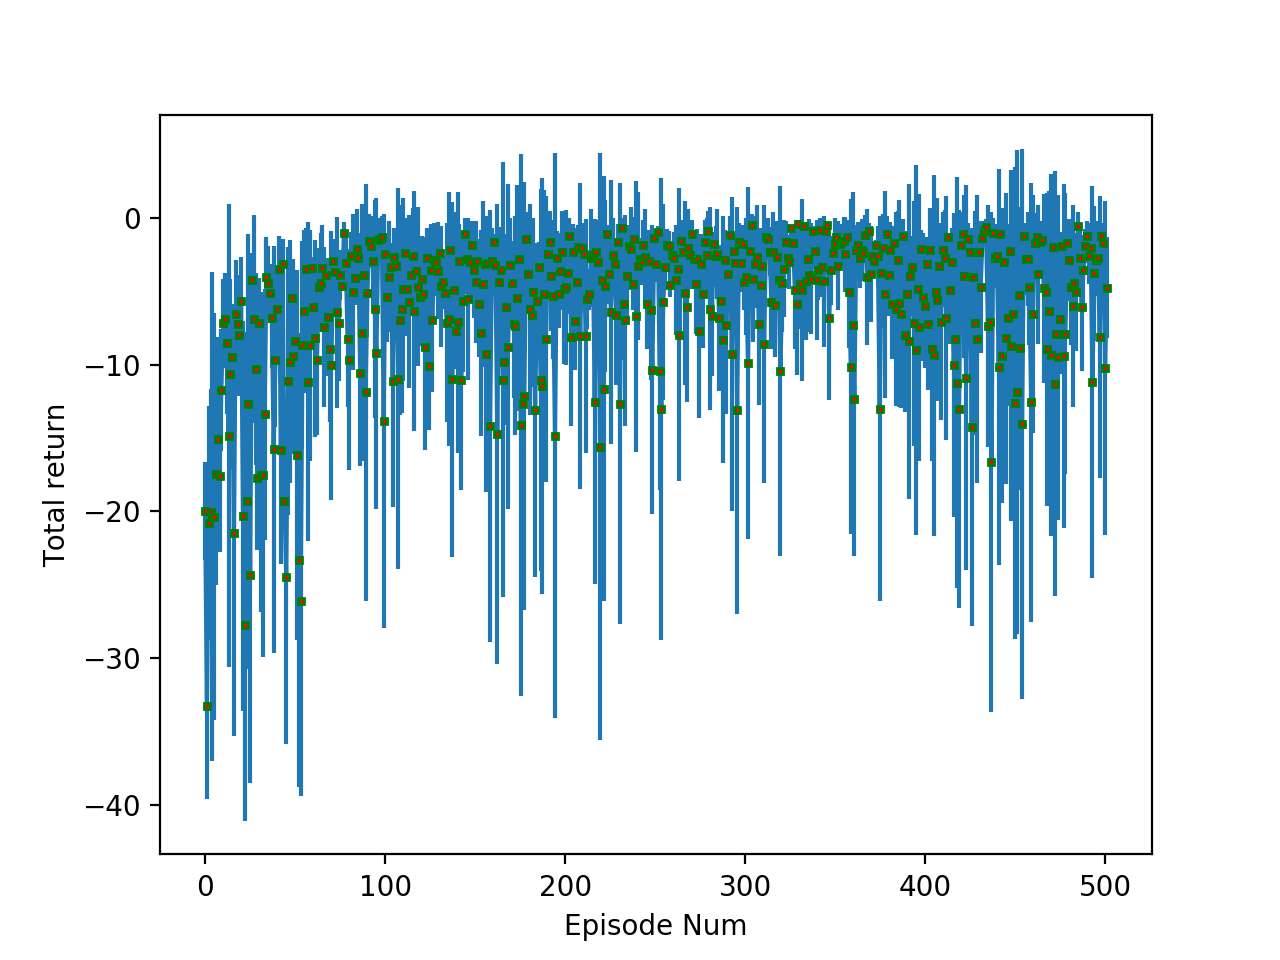
\includegraphics[height=6.0cm,width=9.5cm]{p2.png},
        \caption{Learning Curve for Problem 2}
    \end{figure}
    
    \item (7.5 Points) Repeat the previous question, but using the GA (as described earlier in this assignment) on the More-Watery 687-Gridworld domain. Report the same quantities. \\
    \textbf{Answer:}\\
    Searching strategy is the same. The best hyperparameters are:'sigma': 5.0, 'popSize': 50, 'numElite': 3, 'numEpisodes': 10, 'alpha': 1.0: 30. The learning curve for problem 3 is attached below:
    \begin{figure}[htbp]
        \centering
        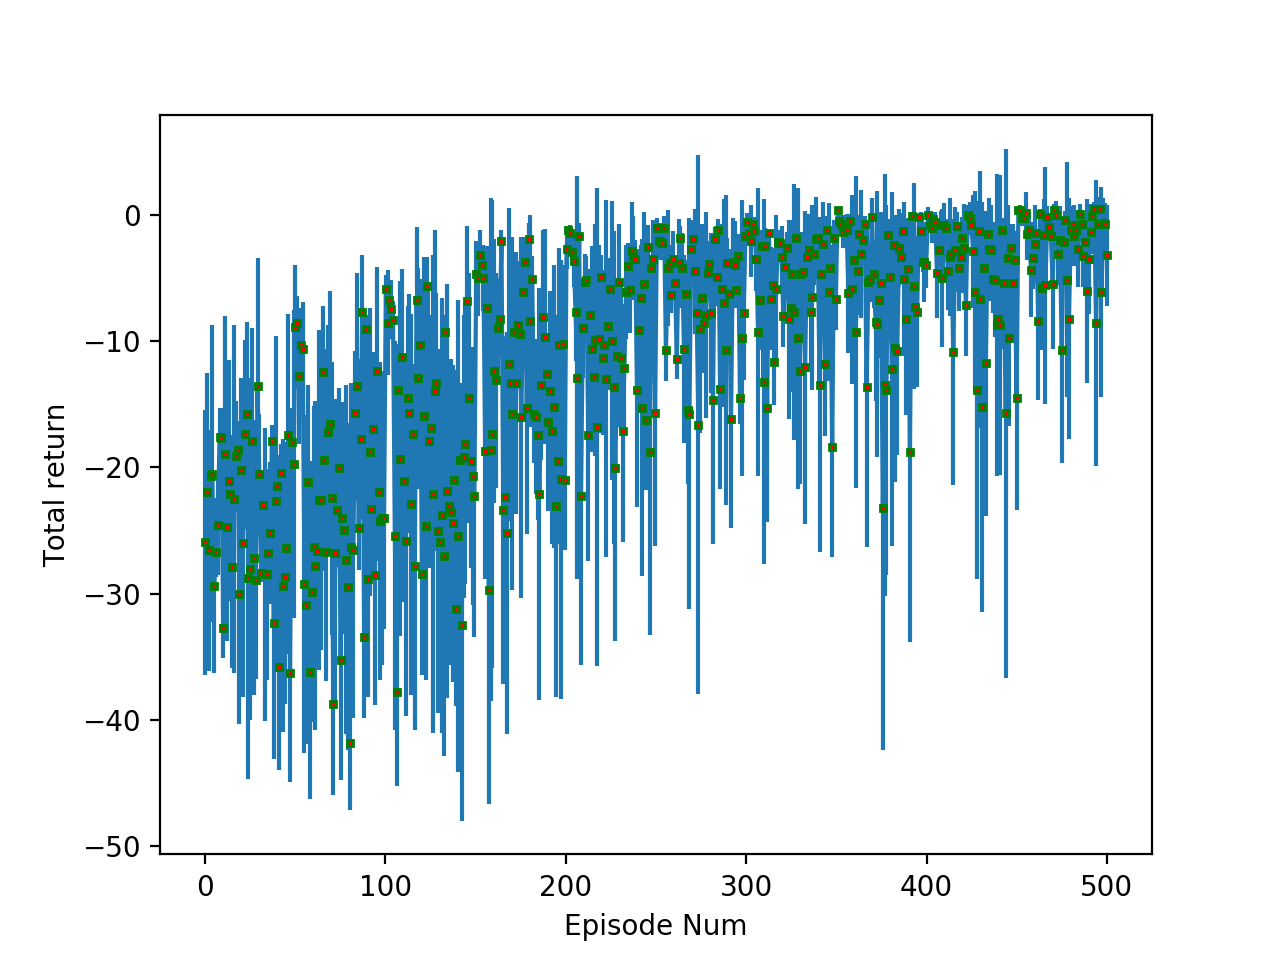
\includegraphics[height=6.0cm,width=9.5cm]{p3.png},
        \caption{Learning Curve for Problem 3}
    \end{figure}
    
    \item (7.5 Points) Repeat the previous question, but using the cross-entropy method on the cart-pole domain. Notice that the state is not discrete, and so you cannot directly apply a tabular softmax policy. It is up to you to create a representation for the policy for this problem. Consider using the softmax action selection using linear function approximation as described in the notes. For descriptions of common choices of $\phi$, see the work of \cite{Konidaris2011}. Report the same quantities, as well as how you parameterized the policy. \\
    \textbf{Answer:}\\
    I used the same searching strategy as before. To parameterize the policy, I mainly referenced the paper cited above. By implementing a fourier transform, we can represent the complex function between states and parameters. The fourier transform using a series of numbers to denote the magnitude for different cos functions with different frequencies, which present a real, continuous problem using discrete methods. Finally a softmax action is used to normalize these values into probabilities used to represent the policy. The best hyperparameters are: 'sigma': 1.625, 'popSize': 40, 'numElite': 4, 'numEpisodes': 30, 'epsilon': 1.475. The learning curve for problem 4 is attached below:
    \begin{figure}[htbp]
        \centering
        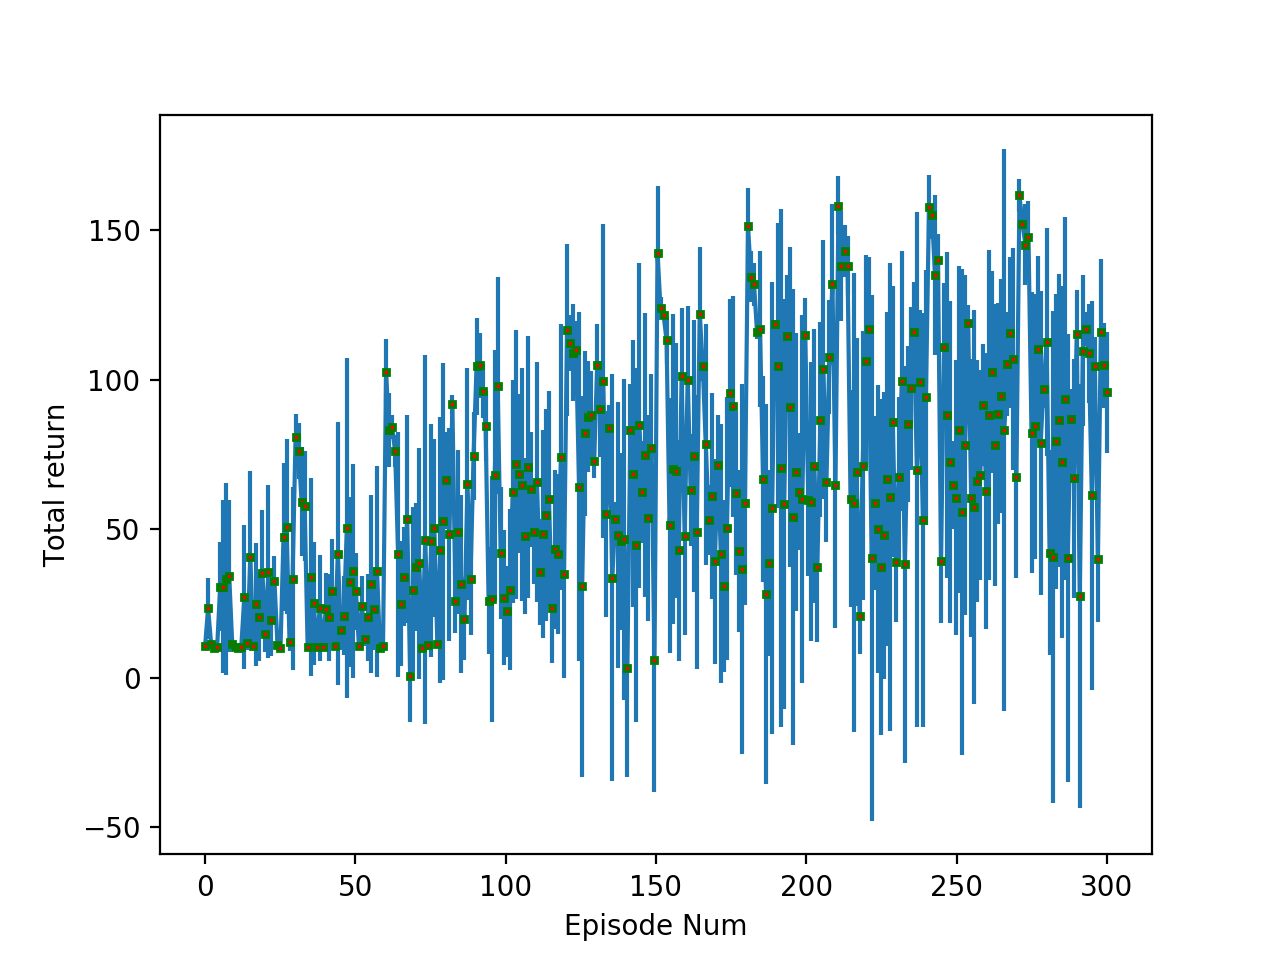
\includegraphics[height=6.0cm,width=9.5cm]{p6.png},
        \caption{Learning Curve for Problem 4}
    \end{figure}

    
    \item (7.5 Points) Repeat the previous question, but using first-choice hill-climbing (as described in class) on the cart-pole domain. Report the same quantities and how the policy was parameterized. \\
    \textbf{Answer:}\\
    Searching strategy is the same. The best hyperparameters are: 'sigma': 1.725, 'numEpisodes': 35. The learning curve for problem 5 is attached below:
    \begin{figure}[htbp]
        \centering
        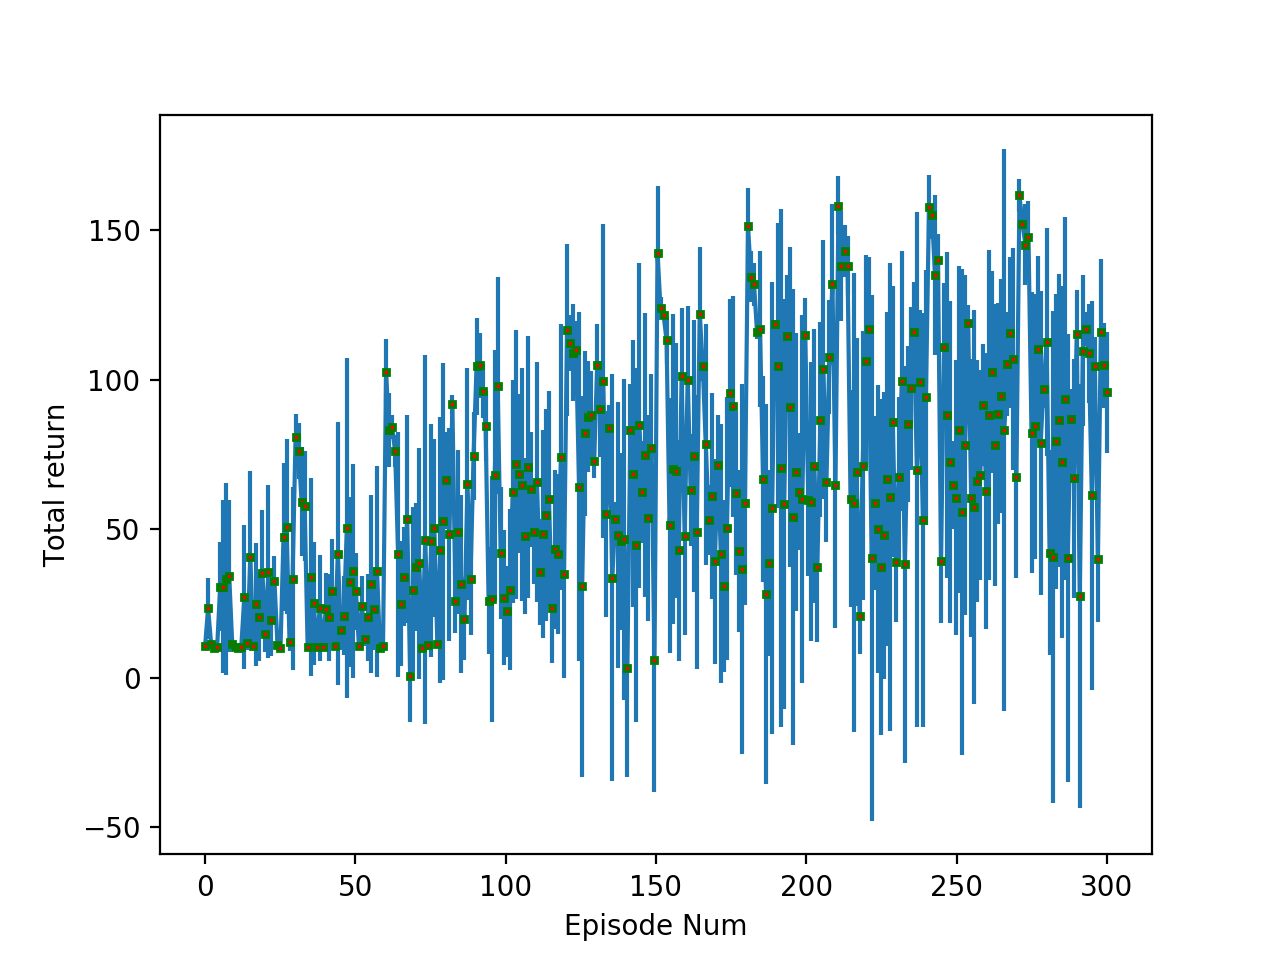
\includegraphics[height=6.0cm,width=9.5cm]{p6.png},
        \caption{Learning Curve for Problem 5}
    \end{figure}

    
    \item (7.5 Points) Repeat the previous question, but using the GA (as described earlier in this homework) on the cart-pole domain. Report the same quantities and how the policy was parameterized. \\
    \textbf{Answer:}\\
    Searching strategy is the same. The best hyperparameters are: 'sigma': 1.625, 'popSize': 30, 'numElite': 4, 'numEpisodes': 40, 'alpha': 2.5. The learning curve for problem 6 is attached below:
    \begin{figure}[htbp]
        \centering
        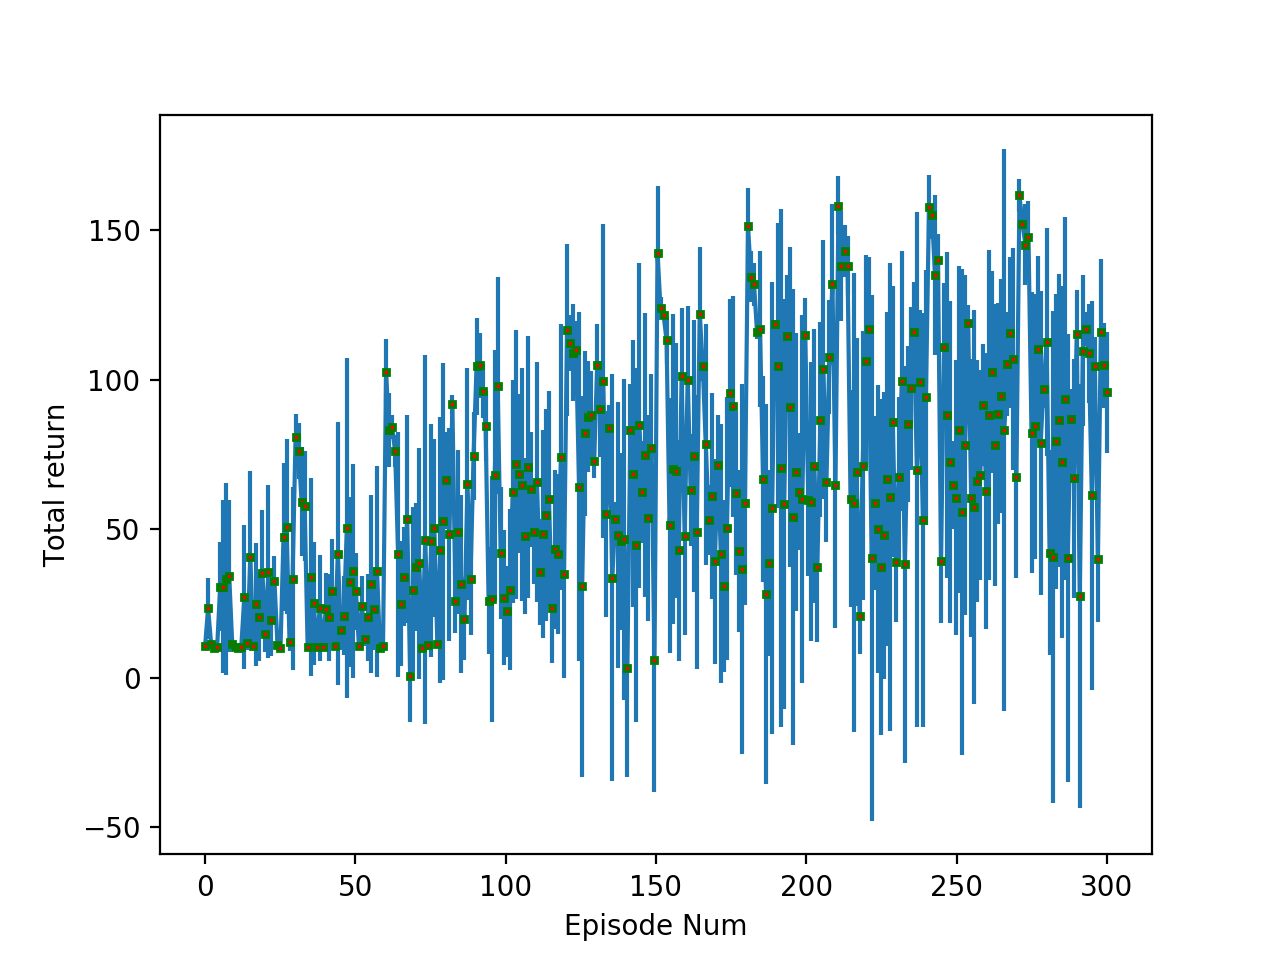
\includegraphics[height=6.0cm,width=9.5cm]{p6.png},
        \caption{Learning Curve for Problem 6}
    \end{figure}


    \item (5 Points) Reflect on this problem. Was it easier or harder than you expected to get these methods working? In the previous assignment you hypothesized how long it would take an agent to solve the More-Watery 687-Gridworld problem. Did it take more or fewer episodes than you expected? Why do you think this happened?\\
    \textbf{Answer:}\\
    It is a little bit harder to implement the linear policy. The fourier transform used here is more abstract than other concepts. For the other problems, the implementation is relatively easier while searching for best hyperparameters is extremely time consuming. I estimated it should take about over 100 episodes last time, and the result shown here is approaximating except for the CEM algorithm. That took a little bit longer to converge. This can be caused by the hyperparameters and the learning rate we assigned in these algorithms.
\end{enumerate}

\bibliography{mybib}
\bibliographystyle{abbrvnat}	% Uses author initials (requires abbrvnat.bst)

\end{document}